\documentclass{article}
\usepackage[utf8]{inputenc}

\title{\underline{\textit{\Large{EE2703: ENDSEMESTER EXAMINATION}}}}
\author{\textit{ROHIT KUMAR, EE20B111}}
\date{May 12, 2022}

\usepackage{natbib}
\usepackage{graphicx}
\usepackage{amsmath}
\usepackage{listings}

\begin{document}

\maketitle

\section{Abstract}
\begin{itemize}
\item To find the antenna currents in a half-wave dipole antenna using:

(i) Standard Expression.
(ii) Magnetic Vector Potential and approximating
\item To study the difference between the graphs obtained via estimation and actual values
\end{itemize}

\section{Introduction}
We have a long wire carrying a current I(z) in dipole antenna with half length 0f 50cm(=l)
so, wavelength = 2m. Next, we need to determine the currents in the two wires of the antenna. Next, we have the expressions to calculate the value of currents.
$$I = I_{m}sin(k(l-z)) $$ $$  0\leq z \leq l$$
$$I = I_{m}sin(k(l+z)) $$ $$  -l\leq z < 0 $$


In the next process, we calculate the magnetic vector potential by approximating the integrals (in terms of summation); we next find out $P_{ij}$ and $P_{B}$.
$$A_{z,i} = \sum_{j}P_{ij}I_{j} + P_{B}I_{N} = \sum_{j}I_{j}(\frac{\mu_{0}}{4\pi}\frac{exp(-jkR_{ij})}{R_{ij}}dz'_{j})$$

$$P_{B} = \frac{\mu_{0}}{4\pi}\frac{exp(-jkR_{iN})}{R_{iN}}dz'_{j}$$

Then, we use the Ampere's circuital law to calculate $H_{\phi}$. Again, we get it in terms of some summation involving the matrices $Q_{ij}$ and $Q_{B}$. 
$$H_{\phi}(r,z_{i}) = \sum_{j}Q_{ij}J_{j} + Q_{Bi}I_{m} = -\sum_{j}P_{ij}\frac{r}{\mu_{0}}(\frac{-jk}{R_{ij}} - \frac{1}{R^2_{ij}}) + P_{B}\frac{r}{\mu_{0}}(\frac{-jk}{R_{iN}} - \frac{1}{R^2_{iN}})$$


At last we solve the matrix equation to find out the current vector \bold{J} and then find out \bold{I}.
$$MJ = QJ + Q_{B}I_{m}$$


\section{Assignment questions}

\subsection{Question 1}
According to the question, we now need to find vector $z$ and $u$. And then find the current vectors $I$ (at loactions of $z$) and $J$ (at locations of $u$) respectively.

\newline The following code snippet does the job!
\begin{verbatim}
z = linspace(-l, l, 2*N + 1)
print(z)

# Calculating I vector(standard expression) - the actual I
I0 = array(np.zeros(2*N + 1)) # Initialisation

# Using the given expressions
I0[0:N] = Im * np.sin(k*(l + z[0:N])) # For -l < z < 0
I0[N:2*N + 1] = Im * np.sin(k*(l - z[N:2*N + 1])) # For 0 < z < l 

# Applying the given boundary condititons
I0[N] = Im
I0[0] = 0
I0[2*N] = 0 
print(I0)

# Calculating u vector
u_index = array(range(1, 2*N))

# Removing the middlemost element
u_index = delete(u_index, N - 1)

u = z[u_index] # Final "u" vector
print(u)

# Calculating J vector - Actual
J0 = I0[u_index] # Excluding the first, middle and extreme values of I0 using the array u
print(J0)
\end{verbatim}
\begin{verbatim}
The values obtained after running the code are:

z = [-0.5  -0.38 -0.25 -0.12  0.    0.12  0.25  0.38  0.5 ]
I0 = [0.   0.38 0.71 0.92 1.   0.92 0.71 0.38 0.  ]
u = [-0.38 -0.25 -0.12  0.12  0.25  0.38]
J0 = [0.38 0.71 0.92 0.92 0.71 0.38]

\end{verbatim}


\subsection{Question 2}
After applying the ampere's circuital law, we can represent all the values in a compact matrix equation: $$H=M*J$$ .
Here, the $M$ is a scaled version of identity matrix: $$M = \frac{I}{2\pi a}$$
where, $I$ is the identity matrix.

Now, the below code snippet is used to implement the above:

\begin{verbatim}
    # Function to compute and return matrix M, H_phi
    def Q2_make_matrices(N, J):
    M = (1/(2*pi*a))*(identity(2*N - 2, dtype = float))
    H = dot(M, J)    
    return M, H     

    M, H = Q2_make_matrices(N, J0) # Getting the matrix M
    print(M.round(2)) 
    
The matrix M obtained is: 
[[15.92  0.    0.    0.    0.    0.  ]
 [ 0.   15.92  0.    0.    0.    0.  ]
 [ 0.    0.   15.92  0.    0.    0.  ]
 [ 0.    0.    0.   15.92  0.    0.  ]
 [ 0.    0.    0.    0.   15.92  0.  ]
 [ 0.    0.    0.    0.    0.   15.92]]
\end{verbatim}


\subsection{Question 3}
After simplifying the vector potential in terms of integration, we now calculate the vectors $Rz$ and $Ru$ and matrices $P$ and $P_{B}$.
The code snippet is as follows:

\begin{verbatim}
def Q3_compute_vectors(N, r):
    zi, zj = meshgrid(z, z) # Returns coordinate matrices from coordinate vectors
    unity_matrix = ones([2*N + 1, 2*N + 1]) 
    Rz = sqrt((r**2*unity_matrix) + (zi - zj)**2) # R^2 = (r^2) + (zi - zj)^2 

    ui, uj = meshgrid(u, u)
    unity_matrix = ones([2*N - 2, 2*N - 2])
    Ru = sqrt((r**2*unity_matrix) + (ui - uj)**2) 

    return Rz, Ru

Rz, Ru = Q3_compute_vectors(N, a) # As we are evaluating at r = a
print(Rz.round(2))
print(Ru.round(2))

def Q3_make_matrices(N, r):
    
    RiN = Rz[N] 
    RiN = delete(RiN, [0, N, 2*N], 0) # Removing the three elements (first, middle, last) 
    PB = ((u0/(4*pi))*(exp(-1j*k*RiN))*(dz/RiN))
    
    Pij = ((u0/(4*pi))*(exp(-1j*k*Ru))*(dz/Ru)) # Using the given expressions
    return Pij, PB

Pij, PB = Q3_make_matrices(N, a) # At r = a   
print((Pij*1e8).round(2))
print((PB*1e8).round(2))

The values of required matrices and vectors obtained are: 

Ru:  [[0.01 0.13 0.25 0.5  0.63 0.75]
 [0.13 0.01 0.13 0.38 0.5  0.63]
 [0.25 0.13 0.01 0.25 0.38 0.5 ]
 [0.5  0.38 0.25 0.01 0.13 0.25]
 [0.63 0.5  0.38 0.13 0.01 0.13]
 [0.75 0.63 0.5  0.25 0.13 0.01]]

Rz:  [[0.01 0.13 0.25 0.38 0.5  0.63 0.75 0.88 1.  ]
 [0.13 0.01 0.13 0.25 0.38 0.5  0.63 0.75 0.88]
 [0.25 0.13 0.01 0.13 0.25 0.38 0.5  0.63 0.75]
 [0.38 0.25 0.13 0.01 0.13 0.25 0.38 0.5  0.63]
 [0.5  0.38 0.25 0.13 0.01 0.13 0.25 0.38 0.5 ]
 [0.63 0.5  0.38 0.25 0.13 0.01 0.13 0.25 0.38]
 [0.75 0.63 0.5  0.38 0.25 0.13 0.01 0.13 0.25]
 [0.88 0.75 0.63 0.5  0.38 0.25 0.13 0.01 0.13]
 [1.   0.88 0.75 0.63 0.5  0.38 0.25 0.13 0.01]]

P:  [[124.94-3.93j   9.2 -3.83j   3.53-3.53j  -0.  -2.5j   -0.77-1.85j
   -1.18-1.18j]
 [  9.2 -3.83j 124.94-3.93j   9.2 -3.83j   1.27-3.08j  -0.  -2.5j
   -0.77-1.85j]
 [  3.53-3.53j   9.2 -3.83j 124.94-3.93j   3.53-3.53j   1.27-3.08j
   -0.  -2.5j ]
 [ -0.  -2.5j    1.27-3.08j   3.53-3.53j 124.94-3.93j   9.2 -3.83j
    3.53-3.53j]
 [ -0.77-1.85j  -0.  -2.5j    1.27-3.08j   9.2 -3.83j 124.94-3.93j
    9.2 -3.83j]
 [ -1.18-1.18j  -0.77-1.85j  -0.  -2.5j    3.53-3.53j   9.2 -3.83j
  124.94-3.93j]]

P_B:  [1.27-3.08j 3.53-3.53j 9.2 -3.83j 9.2 -3.83j 3.53-3.53j 1.27-3.08j]
\end{verbatim}

\subsection{Question 4}
We now simplify the auxiliary field $H_{\phi}(r, z_{i})$ in terms of matrices $Q_{ij}$ and $Q_{B}$. The code snippet to calculate the told matrices are: 
\begin{verbatim}
Qij = ((-Pij*a)/u0)*(((-1j*k)/Ru) - (1/Ru**2))

RiN = Rz[N] 
RiN = delete(RiN, [0, N, 2*N], 0)  

QB = ((-PB*a)/u0)*(((-1j*k)/RiN) - (1/RiN**2))
print(Qij.round(2))
print(QB.round(2))

The output after running the above code is: 
Q:  [[9.952e+01-0.j 5.000e-02-0.j 1.000e-02-0.j 0.000e+00-0.j 0.000e+00-0.j
  0.000e+00-0.j]
 [5.000e-02-0.j 9.952e+01-0.j 5.000e-02-0.j 0.000e+00-0.j 0.000e+00-0.j
  0.000e+00-0.j]
 [1.000e-02-0.j 5.000e-02-0.j 9.952e+01-0.j 1.000e-02-0.j 0.000e+00-0.j
  0.000e+00-0.j]
 [0.000e+00-0.j 0.000e+00-0.j 1.000e-02-0.j 9.952e+01-0.j 5.000e-02-0.j
  1.000e-02-0.j]
 [0.000e+00-0.j 0.000e+00-0.j 0.000e+00-0.j 5.000e-02-0.j 9.952e+01-0.j
  5.000e-02-0.j]
 [0.000e+00-0.j 0.000e+00-0.j 0.000e+00-0.j 1.000e-02-0.j 5.000e-02-0.j
  9.952e+01-0.j]]
Q_B:  [0.  -0.j 0.01-0.j 0.05-0.j 0.05-0.j 0.01-0.j 0.  -0.j]
\end{verbatim}



\subsection{Question 5}
We now have a matrix equation as shown in introduction portion. After solving the matrix equation we get $J$ and next finally we find out our estimated $I$.
The code snippet to do so is follows:
\begin{verbatim}
Inverse = linalg.inv(M - Qij) # Calculating the inverse of (M-Q)
J = dot(Inverse, QB) # As J = [(M-Q)^-1]QB.Im

# Finding I(expected value of current)
# Adding the three values given in question
I = zeros(2*N + 1, dtype = complex)
I[1:N] = J[0:N-1]
I[N+1:2*N] = J[N-1:2*N-1]
I[N] = Im
print(I)

The output obtained is: 
I:  [ 0.00000000e+00+0.00000000e+00j -3.30256482e-05+1.06463792e-05j
 -9.54636142e-05+1.15207845e-05j -6.48254232e-04+1.20785421e-05j
  1.00000000e+00+0.00000000e+00j -6.48254232e-04+1.20785421e-05j
 -9.54636142e-05+1.15207845e-05j -3.30256482e-05+1.06463792e-05j
  0.00000000e+00+0.00000000e+00j]
\end{verbatim}

The next step is to plot the graph of actual I and estimated I.
\begin{figure}[h!]
\centering
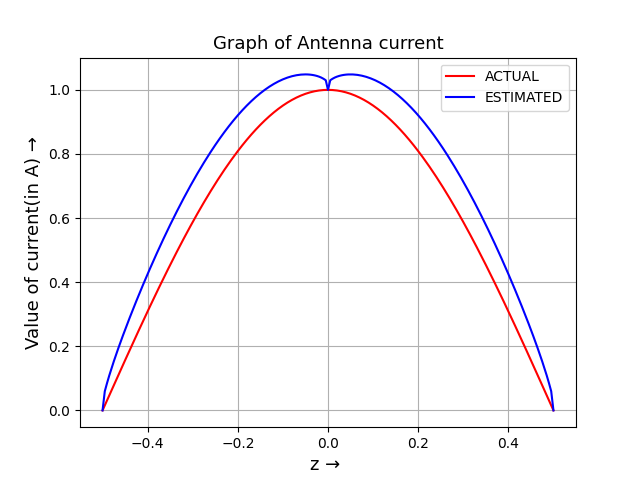
\includegraphics[scale=0.6]{Endsem_2.png}
\caption{Graph of actual and estimated currents}
\label{fig:universe}
\end{figure}

\section{Conclusion}
The following facts can be confirmed after analysing the current for half-wave dipole antenna.

On increasing the value of N,the both graph will merge each other.

• On increasing N,the magnitude of point which are away from the centre
are increasing.
\begin{figure}[h!]
\centering
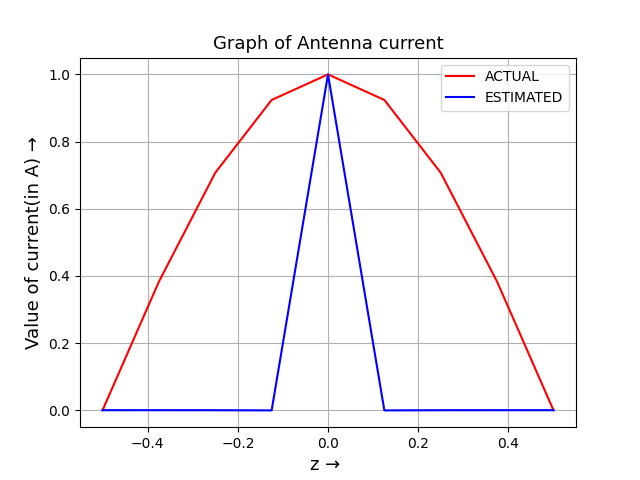
\includegraphics[scale=0.6]{Endsem_1.png}
\caption{Graph of actual and estimated currents for N=4}
\label{fig:universe}
\end{figure}

\begin{figure}[h!]
\centering
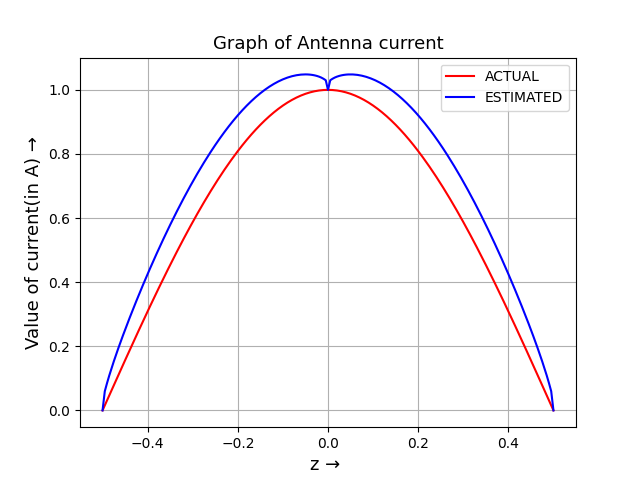
\includegraphics[scale=0.6]{Endsem_2.png}
\caption{Graph of actual and estimated currents for N=100}
\label{fig:universe}
\end{figure}
It is also clear that as number of samples(N) increases, accuracy increases.



\end{document}